\section*{Methods}

The focus of this study is long-trip accessibility for road vehicles. The metric proposed reflects the ease with which a given individual, driving a given vehicle, can access the important locations in a region from one-another. It is assumed that travelers, when considering non-routine long trips have a specific destination in mind and would not consider nearly equivalent and/or equidistant locations as fungible. Rather, having determined to travel to a given location the traveler will then select a mode. Accessibility is a function of demand and impedance. Demand can be estimated by considering the relative attractiveness of given cities as a function of population, economy, or some other metric. Impedance can be quantified by calculating the mode and person specific lowest-cost-paths for all pairs of selected locations within the region and taking the average. Example costs which might be used are travel time and travel price.

A transportation accessibility metric should have land-use, transportation, temporal, and individual components \cite{Karst_2003}. The metric proposed contains all required components. The land-use within a region has two principle effects. First, for a multi-city region, peripheral cities should experience worse regional access than central cities. Second, geographically large and/or sparse regions should experience worse overall accessibility than compact regions. The transportation infrastructure determines the efficacy of various modes. Where only vehicular travel is concerned, the mode choice is reduced to vehicle choice. Vehicle specific infrastructure is not necessarily the same for all vehicles of a given fuel type but is necessarily different between fuel types creating effectively separate modes. The temporal component arises from the schedules of public transportation services and road traffic patterns. Finally the individual component is the traveler risk attitude and route cost weights.

\subsection*{Metric Definition}

Regional travel is often modeled using gravity models. Gravity models theorize that the attraction between two entities is in proportion to the general attractiveness of each and the intervening distance. The units of the resulting attraction have no physical meaning. A region where the sum or average attraction is higher will be a more integrated region. Being concerned with regional performance, this study proposes the Regional Gravity metric $G_R$. For region $R$ of $N$ nodes $O = \{O_1, O_2, \dots, O_N\}$ and a corresponding set of importance weights $W = \{W_0, W_1, \dots, W_N\}$, $G_R$ is computed as

\begin{equation}
	G_{R} = \frac{1}{N^2}\sum_{i = 0}^{N} \sum_{j = 0 }^{N} \frac{CW_iW_j}{Z_{i,j}^2} \label{eq:regional_gravity}
\end{equation}

\noindent where $Z_{i,j}$ is the cost of the optimal path from $O_i$ to $O_j$ and C is a constant tunable parameter. The Specific Regional Gravity $G_{R,i}$ at any node in region $R$ can be computed as

\begin{equation}
	A_{R,i} = \frac{1}{N}\sum_{j = 0 }^{N} \frac{CW_iW_j}{Z_{i,j}^2} \label{eq:specific_regional_accessibility}
\end{equation}

for origin $O_i \in O$. Generally, $W$ will be the set of population masses for each location $M = \{M_0, M_1, \dots, M_N\}$. All else being equal, regions which are more populated/productive, more compact, and enjoy better transportation networks will experience higher $G_R$. This quantity will vary within the region. This study is primarily concerned with the transportation system which contributes directly to arc traversal cost rather than arc demand. Thus a second metric, Regional Impedance is defined as

\begin{equation}
	Z_{R} = \frac{1}{N^2}\sum_{i = 0}^{N} \sum_{j = 0 }^{N} Z_{ij} \label{eq:regional_impedance}
\end{equation}

for region $R$. Specific Regional Impedance $Z_{R,i}$ is defined as

\begin{equation}
	Z_{R,i} = \frac{1}{N}\sum_{j = 0 }^{N} Z_{ij} \label{eq:specific_regional_impedance}
\end{equation}

for a single origin. The Regional Impedance is the average cost of traversing an arc between nodes in a region. Any increase to $Z_R$ would result in a decrease to $G_R$.

\subsection*{Metric Computation}

Powered vehicles are range-limited due to the finite capacity of their \glspl{ess}. In order to traverse an \gls{od} arc whose energy requirement is greater than a vehicle's \gls{ess} capacity, the vehicle must stop at a supply station. In practical terms, the limit is defined by the vehicle's \gls{ess} capacity, starting \gls{soc}, desired finishing \gls{soc}, and the driver's low \gls{soc} tolerance. Because supply events add time to a trip, they will usually be avoided where possible. For sufficiently long trips, where at least one supply event is necessary, computing the shortest-time path requires considering the time added during supply events and the time required to deviate to supply stations. For \glspl{icev}, supply events are brief and supply stations are ubiquitous in most areas of the developed world. Thus, conventional routing services often neglect supply considerations. For \glspl{bev}, supply events are relatively lengthy and DC supply stations are comparatively rare. Ignoring supply events when computing a shortest-time path for a \gls{bev} carries non-negligible risk of a lengthy stop or an out-of-charge event. For this reason, dedicated \gls{bev} routing services such as A Better Route Planner compute routes considering supply events.

All drivers deal with uncertainty and latency issues when computing an optimal route. Certain categories of disruption such as traffic, accidents, supply equipment functionality, and supply equipment local demand cannot be precisely known at the start of the trip. This uncertainty will cause different drivers to evaluate the same arc differently and may result in the selection of different routes. Compounding uncertainty is latency. Although a driver may have access to on the current state of roads and stations to be encountered in the future this may provide little information about conditions upon arrival. Without the ability to reserve a slot at a supply station, drivers cannot be certain of equipment availability until they physically arrive at the station. As such, drivers have to, and do actually, optimize an expectation of route costs when selecting routes. Such optimization may take the form of electing to take a longer ring highway to avoid city traffic, stopping for fuel more often in a sparsely populated area, sitting through a traffic jam rather than diverting, or any number of other strategies. This mental process is modeled via stochastic optimization.

\subsubsection*{Stochastic Optimal Routing}

The purpose of stochastic optimal routing is to find lowest-expected-cost paths from origin $i \in V$ to a set of destinations $D \in V$ on graph $G = \{V, E\}$. The output is tree $P$ containing the optimal-feasible paths from the origin to the selected destinations. The objective of routing on arc $(i,j)\ i, j \in V$ is

\begin{equation}
	\min_{U \in \overline({U}_{i,j})}\ \mathbb{E}[J(S_0, U)]
\end{equation}

where

\begin{equation}
	J(U) = \sum_{k = 0}^M \Phi_k(S_0, U)
\end{equation}

s.t.

\begin{gather}	
	b^k_l \leq \mathbb{E}\left[\int_0^t \Phi_k(S_0, U)dt\right] \leq b^k_u\\
	\mathbb{E}\left[\int_0^T \Phi_k(S_0, U)dt\right] \geq b^k_f\\
	t \in [0, T]\quad k = 1, 2, \dots, M
\end{gather}

\noindent where $T$ is the final value of time for a route, $S$ is the state vector, $S_0$ is the initial values of the states, $U$ is a control (route) between $i$ and $j$, $\overline{U}_{i,j}$ is the set of possible routes between $i$, and $j$, $\Phi$ is the set of cost functions, $b^k_l$ and $b^k_u$ are the upper and lower bounds for state $k$ respectively, and $b^k_f$ is the final state minimum value for state $k$. $\mathbb{E}$ denotes an expectation. State vector $S$ is initialized and stored as vectors containing $N$ discreet variables. A distribution $D$ for a the state vector at any node and time-step can be computed from a histogram of the values. Routes are considered feasible if state expectations remain within set bounds. Comparison between routes is performed using cost expectation.

For vehicle routing, common states are time, distance, price, number of stops, and remaining range. Limits are, often, placed on states and these may not be violated at any time. Limits may also be placed on the final value of a state. Time, distance, price, and number of stops are examples of metrics of minimization which may be used individually or in combination. Upper limits may be set on metrics of optimization in order to terminate the optimization when it is no longer possible to find a feasible route. Remaining range will, necessarily, be subject to upper and lower limits and may be subject to a final value limit (an example of this would be preserving enough range for a return trip).

The values of states are static at nodes and are changed in the process of traversing edges. Intuitively, if a vehicle has 50 km or remaining range at node $i$ and traverses edge $(i, j)$ of distance 20 km ($\Phi_d(i,j) = 20$) then it will arrive at node $j$ with 30 km of remaining range. If node $j$ contains a supply station then range can be added before progressing further. Adding range will cost time and money and should, therefore, be done sparingly. In order to progress from node $j$ to node $k$, the vehicle needs only sufficient range to avoid violating the associated lower bound, in this case 10 km. If $\Phi_d(j,k) \leq 20$ then no resupply is needed. If $\Phi_d(j,k) > 20$ then a resupply event is needed and should add only enough range to make $(j,k)$ feasible. Thus the cost of traversing $(j,k)$ depends on whether or not and how much resupply is needed. 

The extent to which range can be added via resupply is limited by the capacity of the vehicle's \gls{ess} and remaining range constraints. Certain edges will be infeasible regardless of supply as a result. In addition, supply will not be available at all nodes and the cost of supply is neither guaranteed to be homogeneous throughout a network nor to be linear with respect to range added.

The structure of the optimization process is as follows. First, a graph is created to represent the supply network and its interactions among itself and with origins and destinations of interest. All arcs which are feasible should be included as edges in this graph, including those directly between origins and destinations. This graph is described in the \gls{sng} subsection. Second, edge costs in terms of problem states are assigned using models which will be described in the Driver Model, Vehicle model, and Supply Station Model subsections. Third, stochastic optimization is performed using an optimal routing algorithm such as the Dijkstra or Bellman-Ford algorithm.

\subsubsection*{Supply Network Graph}

Supply networks effect routing both in structure and in the characteristics of individual stations. In this paper, the supply network refers to all stations which the vehicle can utilize.Supply networks ultimately consist of individual supply ports (chargers or fuel pumps) and serve geographically and temporally distributed demand. A network consisting of more than one port can develop redundancy either by concentrating ports in a single confined space "in-station" or via a more evenly distributed approach "between-station". Network redundancy also varies by location with "thinner" and "thicker" coverage areas.

The physical connection between supply stations is provide by the road network. Without consideration of range, each station, origin, and destination is reachable from all others. The \gls{sng} is formed from these nodes. Edges are created for all origins and destinations based on shortest paths computed on the road map. Only the locations of and relationships between relevant nodes are necessary. The graph formed from the relevant nodes and their relationships is a reduced subgraph with a low number of nodes and relatively high edges-per-node and cycles-per-node ratios when compared ot the road map.

A reduced subgraph is defined as follows. For a graph $G = \{V, E\}$ where $V$ is the set of nodes and $E$ is the set of edges, a reduced subgraph $\hat{G} = \{\hat{V}, \hat{E}\}$ can be computed where $\hat{V} \subseteq V$ and $\hat{E} = \{P_{ij}\ \forall\ (i, j)\ \in\ \hat{E}\}$ is the set of shortest-paths between all nodes in $\hat{V}$. An example of a reduced subgraph is shown in Figure \ref{fig:reduced_subgraph}.

\begin{figure}[H]
	\centering
	\begin{subfigure}[t]{.5\linewidth}
		\centering\captionsetup{width = .8\linewidth}
		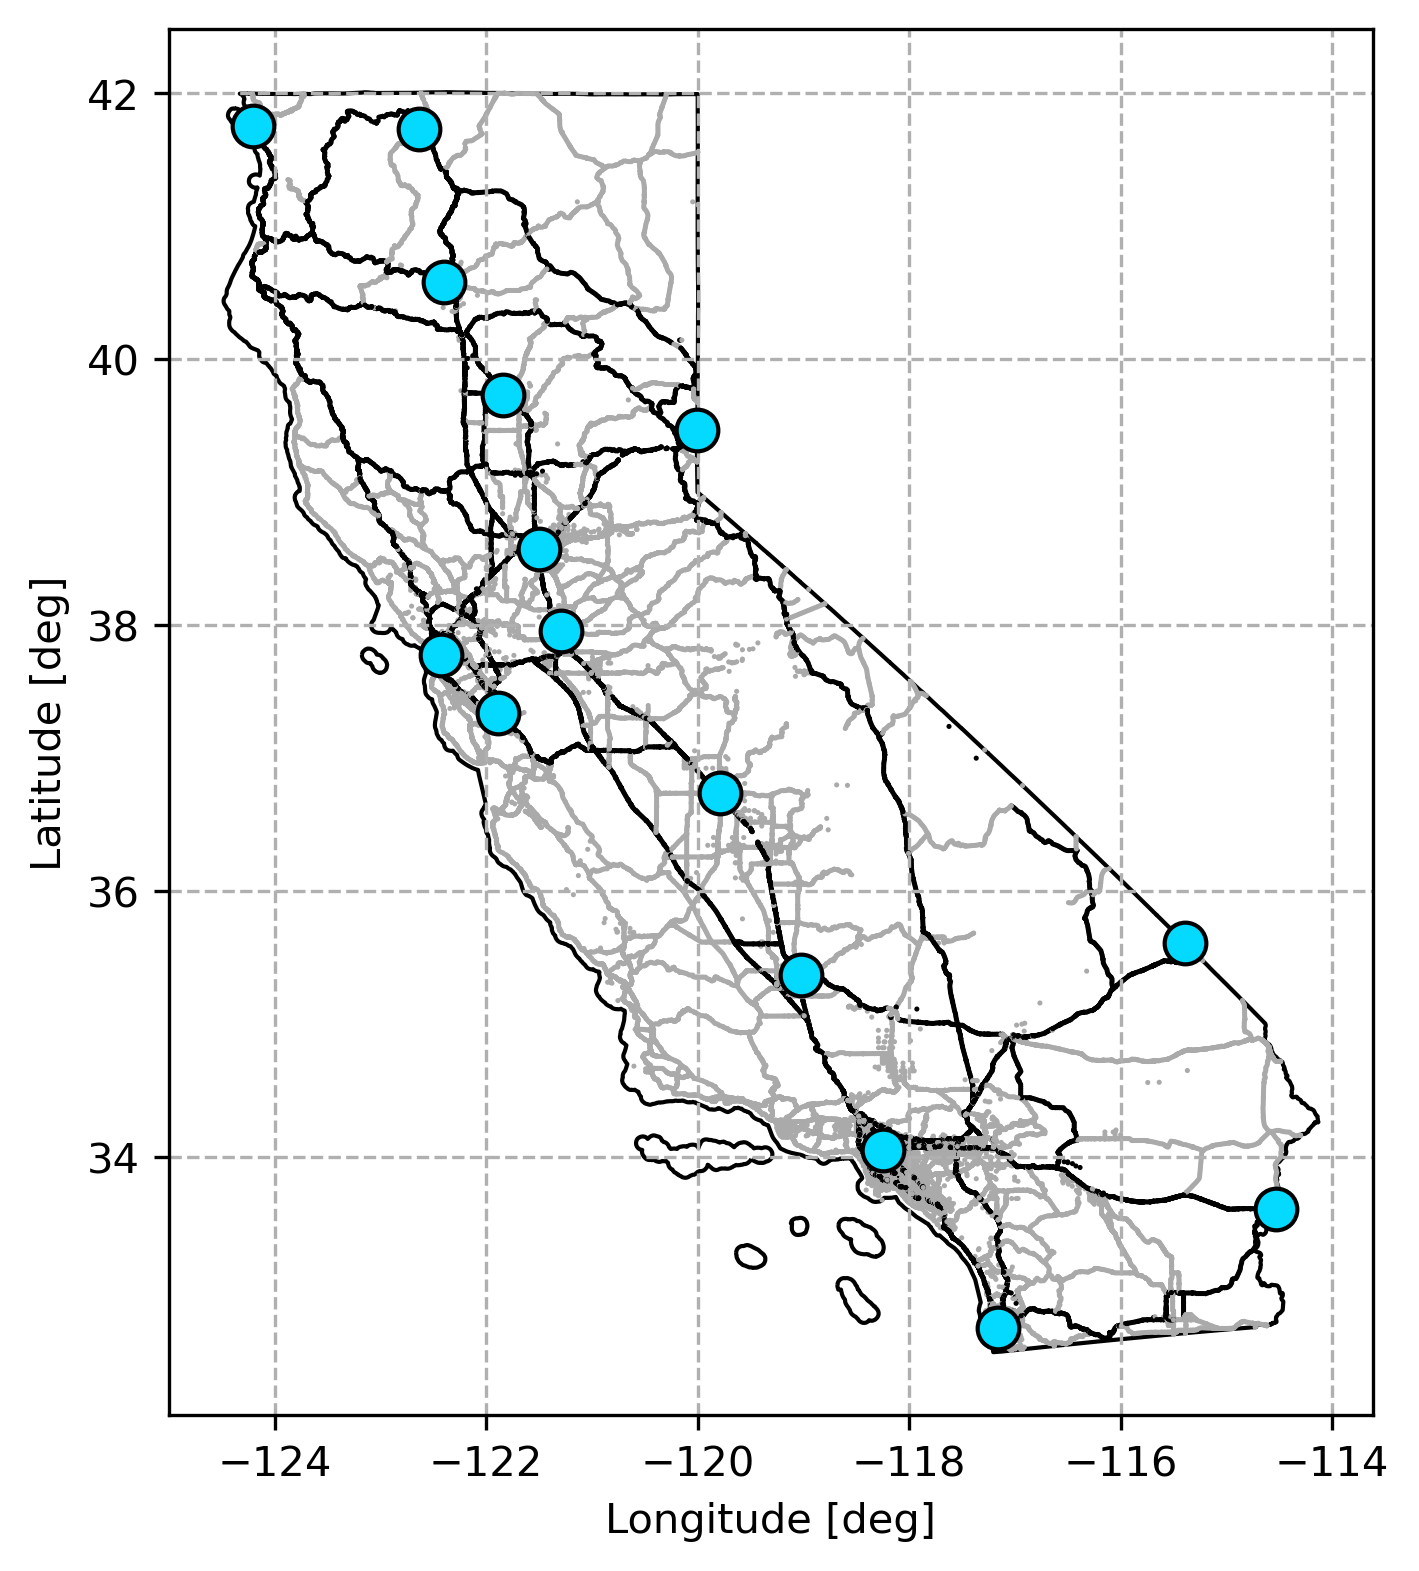
\includegraphics[width = \linewidth]{figs/full_graph.png}
	\end{subfigure}%
	\begin{subfigure}[t]{.5\linewidth}
		\centering\captionsetup{width = .8\linewidth}
		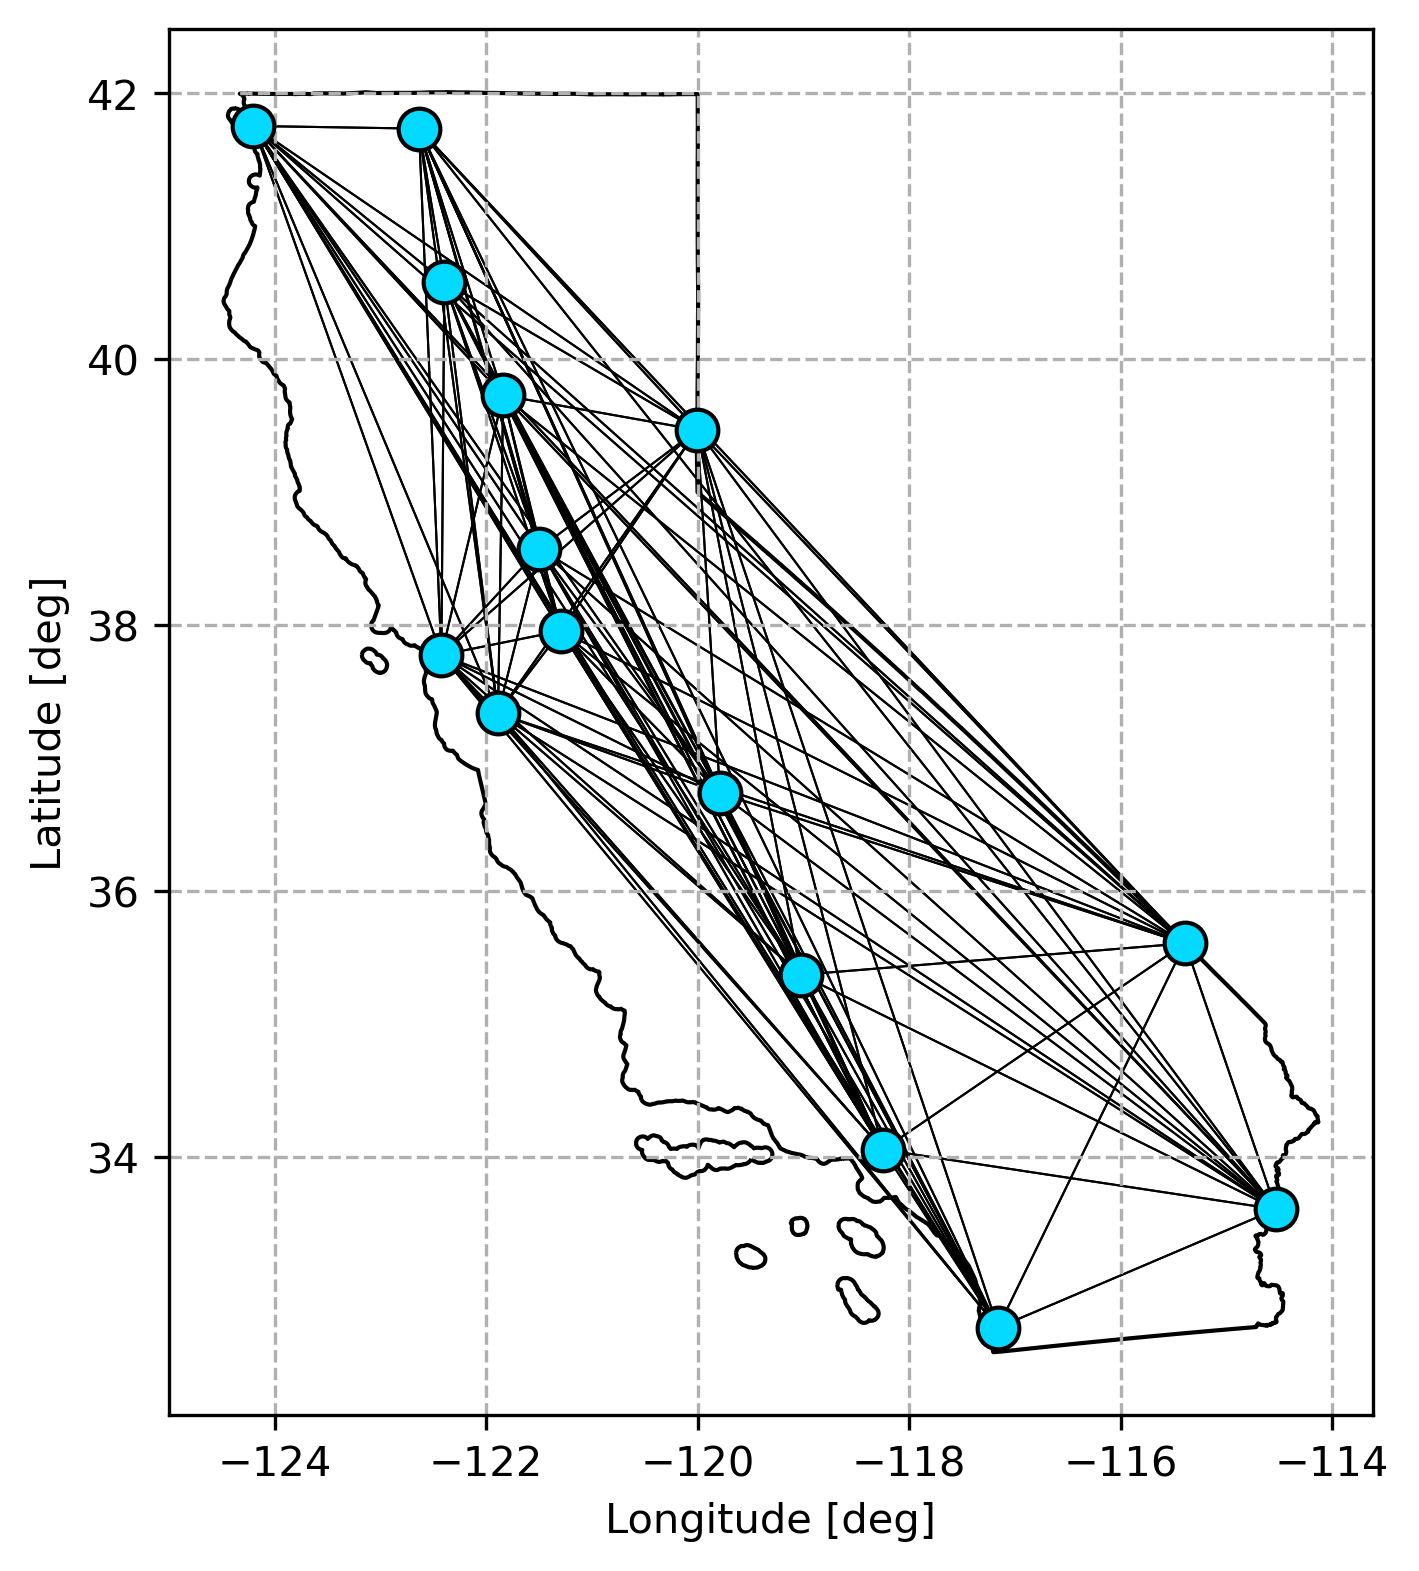
\includegraphics[width = \linewidth]{figs/reduced_graph.png}
	\end{subfigure}
	\caption{Example original graph (left) containing locations and an atlas and reduced subgraph (right) containing locations and arcs.}
	\label{fig:reduced_subgraph}
\end{figure}

Most of the nodes on the \gls{sng} will be supply stations each with different equipment types and numbers of ports. In-station redundancy for a \gls{sng} is a nodal parameter. In-station redundancy $\xi_{is}$ for any node $v \in V$ on \gls{sng} $G = \{V, E\}$ is the number of ports at node $v$. Between-station redundancy $\xi_{bs}$ for an \gls{sng} can be computed for cliques of nodes after solving the maximal clique problem. Between-station redundancy for any clique $C \subseteq V$ on \gls{sng} $G = \{V, E\}$ is the sum of the ports at nodes $v \in C$. Meaningful cliques may be attained by removing edges above a set cost before solving for maximal cliques. For example, cliques may be found on $G' = \{V, E'\}$ where $E' \subseteq E$ contains all edges of less than 10 minutes drive time.

The \gls{sng} is the graph on which long vehicle trips should be optimized if supply events are expensive and/or constraining. The relevant \gls{sng} for \glspl{icev} and \gls{bev} are neither equivalent nor isomorphic. Different vehicles within a given powertrain type may also have different \glspl{sng} but this is far more common for \glspl{ev} than \glspl{icev}. The \gls{sng} informs routing by providing a set of possible paths between origins and destinations. The structure of a network may make for a greater or lesser number of available paths depending on the number and location of stations.

\subsubsection*{Driver Model}

Different drivers will have different perceptions of cost for the same fundamentals based on their priorities and risk attitudes. In a basic sense, drivers will prioritize factors such as time, money, distance, and complexity differently. These priorities are modeled by computing overall cost as a linear combination of individual costs using constant weights. Where any important factor is not known precisely drivers will consider a range of outcomes and decide based on an expectation. Driver risk attitude concerns what range of outcomes will be used to compute expected cost. Risk attitude is modeled using a superquantile risk function defined as

\begin{equation}
	S(D, p_0, p_1) = \frac{1}{p_1 - p_0}\int_{p_0}^{p_1}Q(D, \alpha)\ d\alpha \label{eq:superquantile}
\end{equation}

\noindent where $D$ is a distribution, $p_0$ and $p_1$ are the boundaries of the range of probabilities considered in the expectation, and $Q$ is the quantile function of $D$. The superquantile is, thus, the mean value of a distributed quantity within a range of probability. $S(D, 0, 1)$ reduces to the mean of $D$. Drivers with an aggressive risk attitude will consider a low range of probabilities. Drivers with a neutral attitude will consider a central range of probabilities. Drivers with a cautious attitude will consider a high range of probabilities. Driver parameters are listed in Table \ref{tab:param_driver}.

\begin{table}[H]
	\centering
	\caption{Supply Station Parameters for Routing}
	\label{tab:param_driver}
	\begin{tabular}{|C{\linewidth*3/8}|C{\linewidth*3/8}|C{\linewidth*2/8}|}
		\hline \rowcolor{lightgray} Parameter & Description & Unit \\
		\hline Priorities $W$ & Set of multipliers for route costs to be used in computation of weighted sum & [-] \\
		\hline Risk Attitude $(p_0, p_1)$ & Range of probabilities for superquantile function & [-] \\
		\hline
	\end{tabular}
\end{table}

The driver model serves to bias the routing by selecting a subset of information to use in optimization. As such it reflects individual perception. The results of the routing can be interpreted through the same bias, a different bias, or no bias. In this study, evaluation will be conducted on the basis of un-biased interpretation of costs.

\subsubsection*{Vehicle Model}

Vehicles effect routing due to their range limits and supply methods. The vehicle model used herein is highly simplified due to the inexact nature of the problem. Vehicles are modeled as storing energy and consuming energy at a constant rate per unit distance driven. More exact information on road conditions, traffic conditions, and atmospheric conditions among others can be used to compute edge-specific efficiencies. Vehicular parameters are listed in Table \ref{tab:param_veh}.

\begin{table}[H]
	\centering
	\caption{Vehicle Parameters for Routing}
	\label{tab:param_veh}
	\begin{tabular}{|C{\linewidth*3/8}|C{\linewidth*3/8}|C{\linewidth*2/8}|}
		\hline \rowcolor{lightgray} Parameter & Description & Unit \\
		\hline \gls{ess} Capacity & Accessible energy storage capacity & [kWh] \\
		\hline Energy Consumption & Energy required to move the vehicle & [kJ/km] \\
		\hline Maximum Supply Rate & \gls{ess} maximum energy addition rate & [kW] \\
		\hline Linear Charging Fraction & Percentage of the battery capacity which can be charged in the linear (constant current) range & [kW] \\
		\hline \gls{soc} Bounds & Range in which \gls{soc} must be maintained & [-] \\
		\hline
	\end{tabular}
\end{table}

DC charging is modeled using a CC-CV relationship wherein the first part of charging is linear and the second part follows exponential decay \cite{Marra_2012}. The inflection point which separates the linear and exponential decay sections is the Linear Charging Fraction $\eta$. The time required for a given charge event is

\begin{gather}
	\Delta T = \Delta T_{l} + \Delta T_{e} \\
	\Delta T_{l} = \begin{cases}
		\frac{(SOC_f - SOC_i) C}{\nu} &  SOC_i \leq SOC_f \leq \eta \\
		\frac{(\eta - SOC_i) C}{\nu} &  SOC_i \leq \eta \leq SOC_f \\
		0 &  \eta \leq SOC_i \leq SOC_f
	\end{cases} \\
	\Delta T_{e} = \begin{cases}
		0 & SOC_i \leq SOC_f \leq \eta \\
		-\frac{1}{\alpha}\ln{\left(1-\frac{SOC_f - \eta}{1-\eta}\right)} &  SOC_i \leq \eta \leq SOC_f \\
		-\frac{1}{\alpha}\ln{\left(1-\frac{SOC_f - SOC_i}{1-\eta}\right)} &  \eta \leq SOC_i \leq SOC_f \\
	\end{cases} \\
	\alpha = \frac{\nu}{\eta C}
\end{gather}

Where $C$ is the vehicle \gls{ess} capacity, $\nu$ is the actual power of the charge event, $\Delta T_l$ and $\Delta T_e$ are the time spent in the linear and exponential decay portions of the charge event, and $SOC_i$ and $SOC_f$ are the initial and final values of \gls{soc} for the charge event. Charge events are modeled to occur at the minimum of the maximum powers for the vehicle and charger. A typical value for $\eta$ will be in the range of 0.7 to 0.8. DC charging for a given quantity of energy past $\eta$ will take substantially longer than the same quantity below $\eta$. The difference in effective charging rate may serve to favor more DC charge events in a given arc which terminate at a lower \gls{soc}.

\subsubsection*{Supply Station Model}

Supply station design parameters are number of ports, reliability of ports, and the maximum supply rate of ports. The probability of port availability at a station is determined by the rate at which vehicles arrive at the station and how long they spend at the station. In combination, these factors determine the likelihood of a port being usable and available as well as the likely duration of queue if no port is usable and available. Supply station parameters are listed in Table \ref{tab:param_supply}.

\begin{table}[H]
	\centering
	\caption{Supply Station Parameters}
	\label{tab:param_supply}
	\begin{tabular}{|C{\linewidth*2/8}|C{\linewidth*3/8}|C{\linewidth*3/8}|}
		\hline \rowcolor{lightgray} Parameter & Description & Unit \\
		\hline Supply Rate & Maximum rate of energy supply & [kW] \\
		\hline Ports & Number of chargers/pumps at a station which can be used simultaneously & [-] \\
		\hline Reliability & Percentage of the time that a given pump will be usable & [-] \\ 
		\hline
	\end{tabular}
\end{table}

Information on ports is taken from \gls{afdc} \cite{afdc_2023}, information on equipment reliability is taken from \cite{Rempel_2023}, and information on port supply rates is taken from Google Maps.

Queue waiting time is computed using the M/M/c queuing formula with parametric uncertainty. The expected waiting time in an M/M/c queue is computed as

\begin{gather}
	W_q = \pi_0\frac{\rho(c\rho)^c}{\lambda(1-\rho)^2c!}\\
	\pi_0=\left[\left(\sum_{k = 0}^{c - 1}\frac{(c\rho)^k}{k!}\right) + \frac{(c\rho)^c}{c!(1 - \rho)}\right]\\
	\rho = \frac{\lambda}{c\mu}
\end{gather}

where $\lambda$ is the arrival frequency, $\mu$ is the service completion frequency, $c$ is the number of homogeneous servers, $\rho$ is the ratio of arrival frequency to composite maximum service completion frequency, and $\pi_0$ is the probability of an empty system. M/M/c queues assume an exponential distribution for both arrival and service completion frequency centered on a known mean. Reflecting the lack of information on charger accessibility accessible to drivers, these parameters must be sampled from distributions. Arrival frequency is much more uncertain than service completion frequency for drivers unfamiliar with a station. As such the drivers are modeled as assuming that charge event times will reflect the time required to fulfill a charge event sampled from a normal distribution and then picking values of $\rho$ based on their risk attitudes. In this study, charging event times in minutes are sampled from the normal distribution $N(30, 10)$. The effects of $\rho$ and in-station redundancy are shown in Figure \ref{fig:reduncancy_rho_wq}.

\begin{figure}[H]
	\centering
	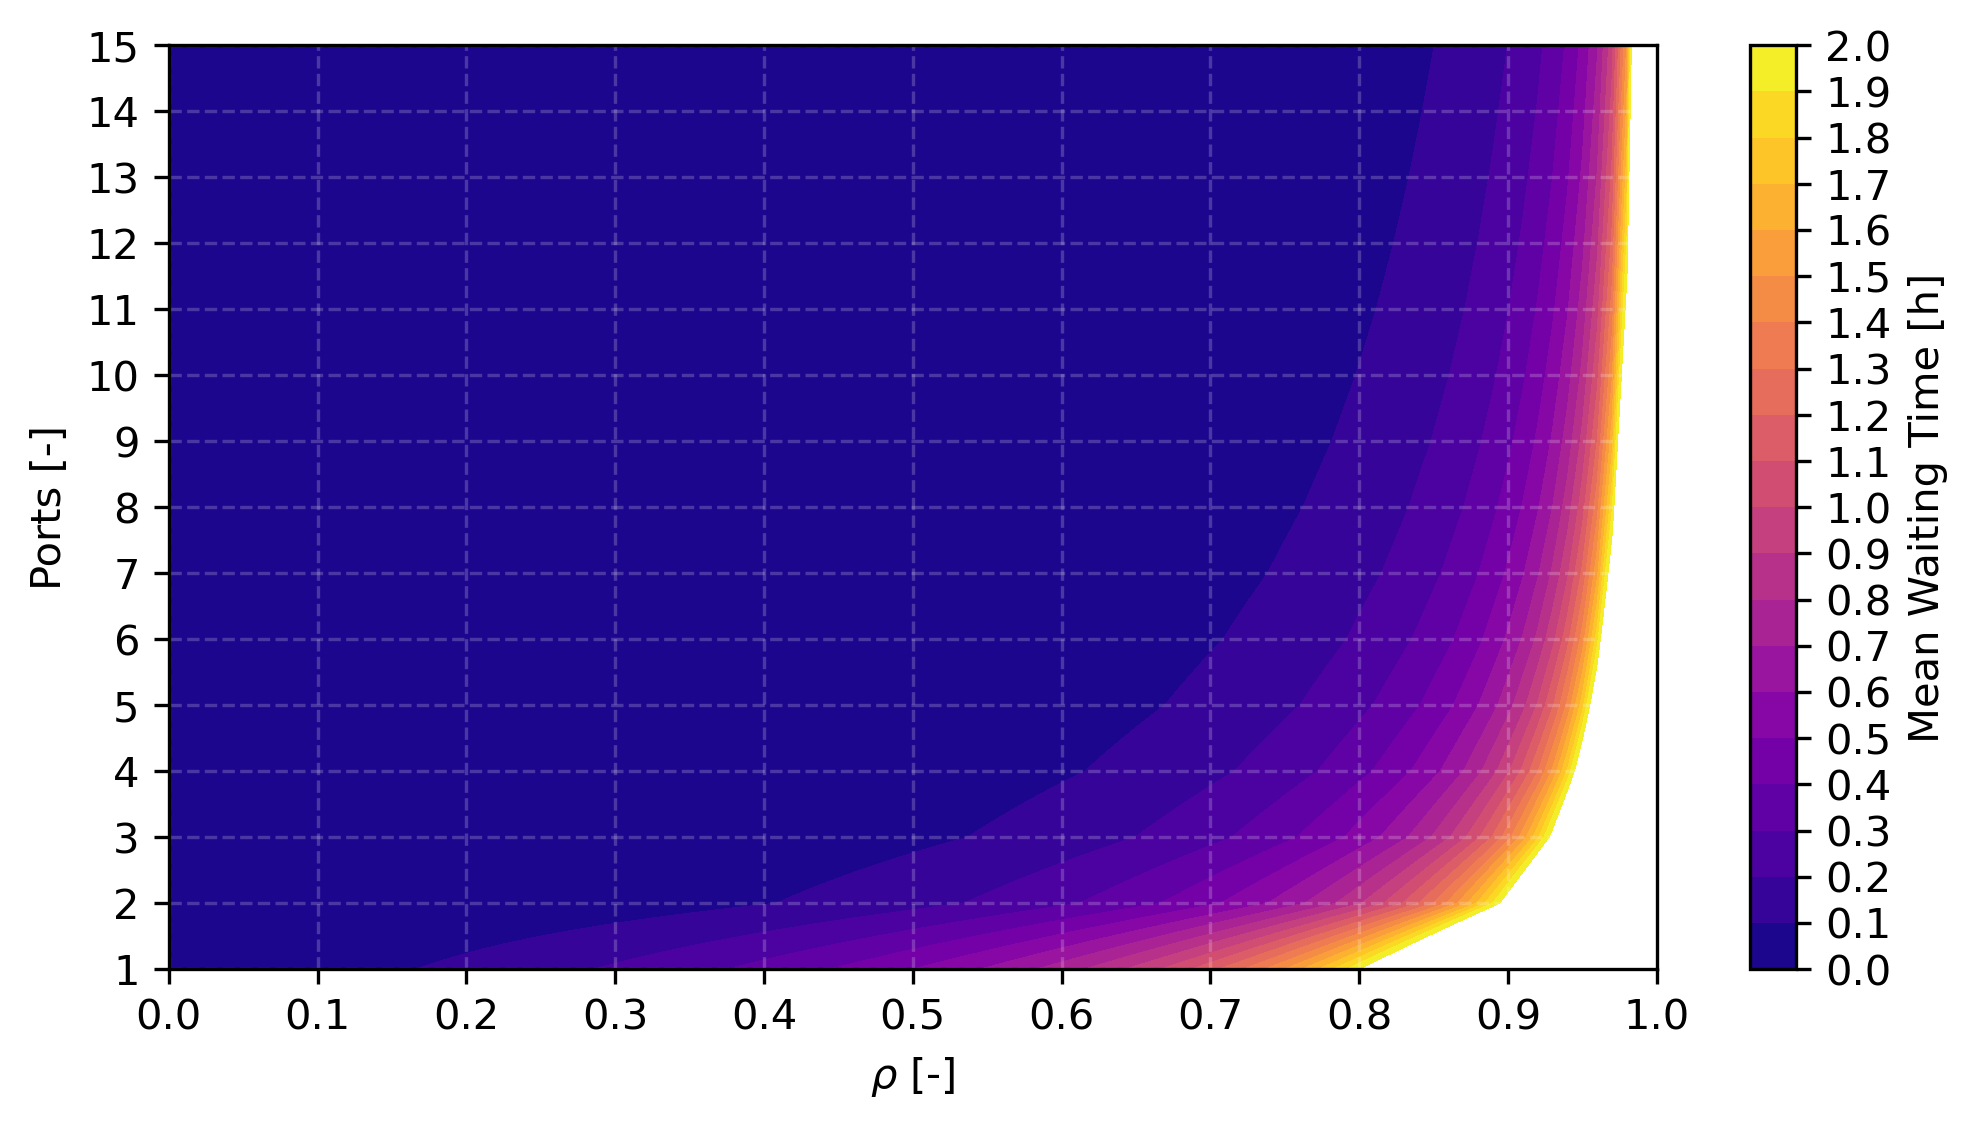
\includegraphics[width = \linewidth]{figs/waiting_time_rho_ports.png}
	\caption{Effects of in-station redundancy and $\rho$ on expected waiting time. Projected times of greater than 2 hours omitted in order to preserve scale.}
	\label{fig:reduncancy_rho_wq}
\end{figure}

Without prior information, a reasonable assumption is that a station will be sized, roughly, to meet demand. The $\rho$ parameter reflects the ratio of demand to maximum capacity and scales with redundancy all else being equal. However, unless completely saturated, a station with more port will be able to handle the same relative demand with a shorter queue due to heterogeneity in individual supply event times. With low demand, durable queues are unlikely to form at any station. As $\rho$ approaches 1, the expected duration of a queue grows toward infinity in a phenomenon known as queue instability. The rate of queue growth as a function of demand growth is determined by redundancy. In practice, a queue of sufficient length will be intolerable to any driver in almost any circumstance limiting queue growth. If this limit is 2 hours then, as seen in figure \ref{fig:reduncancy_rho_wq}, a cautious driver may view 1 and 2 port stations as ineligible.

\subsubsection*{Summary}

The Regional Impedance metric $Z_R$ quantifies the weighted average time of arcs between important locations in a region. $Z_R$ can be computed for any mode or set of modes. For the context of road vehicles, those vehicles which must resupply energy from different networks are, in effect, different modes. $Z_R$ is computed for a driver vehicle by building the relevant \gls{sng} and performing optimal routing based on the drivers preferences and perceptions and the physical characteristics of the vehicle and \gls{sng}. In this study the cost in question is total travel time. The total travel time is the combination of driving time, supply event time, and time spent queuing at supply stations. Each aspect of total travel time must be estimated by the driver with imperfect information when planning a route. Pure driving time is relatively knowable and a decent estimation may be obtained from many routing services. Supply event time is also relatively knowable, especially for experience drivers. Queue waiting time is far less knowable as accurate and timely information on charger utilization and equipment functionality is difficult to come by. Even where it is available beforehand, it may change by the time the driver arrives. These uncertainty and latency issues can substantially increase total travel times. In this study, queue waiting times are estimated by the driver based on the number of ports listed at a station while the actual queue waiting times are computed based on the number of functional ports. When equipment reliability is low drivers may end up spending more time than anticipated, especially if redundancy is also low. In the following case studies $Z_R$ is used as a metric of evaluation to study the impacts of model parameters on transportation accessibility.